\documentclass{article}

\usepackage[utf8]{inputenc}
\usepackage[T1]{fontenc}
\usepackage{amsmath}
\usepackage[framed]{matlab-prettifier}
%\usepackage[a4paper, total={6in, 8in}]{geometry}
\usepackage[a4paper, margin=4cm,top=2cm,landscape]{geometry}
\usepackage[italian]{babel}
\usepackage{pdfpages}


\setlength{\parskip}{5pt}
\setlength{\parindent}{0pt}
\lstset{
style      = Matlab-editor,
basicstyle = \mlttfamily,
%backgroundcolor = \color{lightgray},
numbers=left,
numbersep=5pt,
numberstyle=\tiny\color{gray},
tabsize=2,
morekeywords={yyaxis,abs,logspace,loglog,xlabel,ylabel,figure,exp,title,semilogx,legend,zeros,rand,ones,tic,toc,plot},
frameshape={RYR}{Y}{Y}{RYR},
}


\begin{document}

\section*{Esercizi per l'esame}

\subsection*{Aritmetica Finita - 6}

Come richiesto implementiamo il calcolo del seno iperbolico tramite definizione

\begin{lstlisting}
	naif_sinh = @(x) (exp(x)-exp(-x))./2;
\end{lstlisting}

Adesso calcoliamo l'errore assoluto e l'errore relativo, prendendo come valore di riferimento l'implementazione interna di MATLAB del seno iperbolico. Valutiamo gli errori per valori di $x$ compresi tra ${10}^{-12}$ e ${10}^0$. In particolare evidenzieremo tali errori nei punti $x={10}^{-12} ,{10}^{-11} ,\ldots ,{10}^{-1} ,{10}^0$

\begin{lstlisting}
	asse_x = logspace(-12,0,10*(13-1)+1);
	fine = 1:10:130;
	err_assoluto = abs(sinh(asse_x)-naif_sinh(asse_x));
	err_relativo = err_assoluto./sinh(asse_x);
\end{lstlisting}

Disegnamo infine un unico grafico (con due assi verticali) dove rappresentare gli errori relativi e assoluti.

\begin{lstlisting}
	figure();
	title('Grafico degli errori di sinh(x) - naif');
	yyaxis left;
	semilogx( asse_x,err_assoluto,'-',10.^(-12:0),err_assoluto(fine),'*');
	ylabel('Errore assoluto');
	yyaxis right;
	loglog(asse_x,err_relativo,'-',10.^(-12:0),err_relativo(fine),'*');
	ylabel('Errore relativo (scala logaritmica)');
\end{lstlisting}

Come si può notare nal grafico seguente, l'errore relativo aumenta per piccoli valori di x. Questo è giustificato poichè il numeratore della definizione del seno iperbolico presenta una differenza tra quantità che diventano tanto più prossime quanto più $x$ è piccolo, portando quindi ad un fenomeno di cancellazione numerica.

\includepdf{./Esercizi_images/untitled0.eps}

\clearpage
\subsection*{Aritmetica Finita - 7}

Continuando con i dati dell'esericzio precedente, implementiamo il calcolo del seno iperbolico in modo da evitare fenomeni di cancellazione numerica.

\begin{lstlisting}
	mio_sinh = @(x) (expm1(x)+expm1(x)./(expm1(x)+1))/2;
\end{lstlisting}

Ora calcoliamo e disegnamo il grafico dell'errore relativo di quest'ultima implementazione calcolato rispetto a quella interna a MATLAB

\begin{lstlisting}
	figure();
	mio_err_assoluto = abs(sinh(asse_x)-mio_sinh(asse_x));
	mio_err_relativo = mio_err_assoluto./sinh(asse_x);
	title('Grafico degli errori di sinh(x) - smart');
	yyaxis left;
	semilogx(asse_x,mio_err_assoluto,'-*');
	ylabel('Errore assoluto');
	yyaxis right;
	semilogx(asse_x,mio_err_relativo,'-*');
	ylabel('Errore relativo');
\end{lstlisting}

Come si può notare nel grafico seguente, l'errore assoluto (e quindi quello relativo) sono drasticamente diminuiti, in alcuni punti sono addirittura nulli. Questo indica che l'implementazione alternativa è preferibile per valori di $x$ prossimi a zero.

\includepdf{./Esercizi_images/untitled1.eps}

\clearpage
\subsection*{Aritmetica Finita - 8}

Definiamo, come richiesto, un'espressione matematicamente equivalente alla differenza divisa di ordine uno di $f\left(x\right)=x^3$ ma priva di cancellazione numerica:

\begin{equation*}
	f[x_0,x_0+h]
	%=\frac{f(x_0 +h)-f(x_0)}{h}
	=\frac{{(x_0 +h)}^3 -x_0^3}{h}
	=\frac{x_0^3+3x_0^2 h+3x_0 h^2 +h^3 -x_0^3}{h}
	=3x_0^2 +3x_0 h+h^2
\end{equation*}

Si può notare come l'ultima espressione sia esente da cancellazione numerica in quanto è la somma di sole quantità strettamente positive. Calcoliamo ora i valori delle due differenze divise per specifici valori di $x$ e di $h$

\begin{lstlisting}
	asse_x = logspace(1,4,10*(4-1)+1);
	fine = 1:10:40;
	h = 10^-7;
	differenza_divisa = ((asse_x+h).^3-(asse_x).^3)/h;
	differenza_divisa_no_err = 3*(asse_x).^2 + 3*asse_x*h + h^2;
\end{lstlisting}

Calcoliamo gli errori ed infine disegnamo i grafici richiesti

\begin{lstlisting}
	err_assoluto = abs(differenza_divisa - 3*asse_x.^2);
	err_assoluto_smart = abs(differenza_divisa_no_err - 3*asse_x.^2);
	err_relativo = err_assoluto./abs(3*asse_x.^2);
	err_relativo_smart = err_assoluto_smart./abs(3*asse_x.^2);
	figure();
	loglog( 10.^(1:4),err_assoluto(fine),'bd',...
		10.^(1:4),err_assoluto_smart(fine),'b*',...
		10.^(1:4),err_relativo(fine),'rd',...
		10.^(1:4),err_relativo_smart(fine),'r*',...
		asse_x,err_assoluto,'-b',...
		asse_x,err_assoluto_smart,'-b',...
		asse_x,err_relativo,'-r',...
		asse_x,err_relativo_smart,'-r');
	legend({'AbsErr naif','AbsErr smart','RelErr naif','RelErr smart'},'Location','best');
	title('Errore relativo e assoluto delle differenze divise di x^3');
\end{lstlisting}

\includepdf{./Esercizi_images/untitled2.eps}

\clearpage

Ripetendo lo stesso esercizio con $f\left(x\right)=x^5$ otteniamo

\begin{equation*}
	f[x_0 ,x_0 +h]
	=\frac{f(x_0 +h)-f(x_0 )}{h}
	=\frac{{(x_0 +h)}^5 -x_0^5 }{h}
	=\ldots=
	5x_0^4 +10x_0^3 h+10x_0^2 h^2 +5x_0 h^3 +h^4
\end{equation*}

\begin{lstlisting}
	differenza_divisa        = ((asse_x+h).^5-(asse_x).^5)/h;
	differenza_divisa_no_err = 5*(asse_x).^4 + 10*asse_x.^3*h + 10*asse_x.^2*h^2 + h^4;
	err_assoluto             = abs(differenza_divisa - 5*asse_x.^4);
	err_assoluto_smart       = abs(differenza_divisa_no_err - 5*asse_x.^4);
	err_relativo             = err_assoluto./abs(5*asse_x.^4);
	err_relativo_smart       = err_assoluto_smart./abs(5*asse_x.^4);
	figure();
	loglog(10.^(1:4),err_assoluto(fine),'bd',...
		10.^(1:4),err_assoluto_smart(fine),'b*',...
		10.^(1:4),err_relativo(fine),'rd',...
		10.^(1:4),err_relativo_smart(fine),'r*',...
		asse_x,err_assoluto,'-b',...
		asse_x,err_assoluto_smart,'-b',...
		asse_x,err_relativo,'-r',...
		asse_x,err_relativo_smart,'-r');
	legend({'AbsErr naif','AbsErr smart','RelErr naif','RelErr smart'},'Location','best');
	title('Errore relativo e assoluto delle differenze divise di x^5');
\end{lstlisting}

\includepdf{./Esercizi_images/untitled3.eps}

\clearpage
\subsection*{Vettori, matrici e sistemi lineari - 8}

Viene data una matrice definita così:

\begin{equation*}
A =
\begin{bmatrix}
	A_{11} & A_{12} \\
	0      & A_{22}
\end{bmatrix}
\quad \textrm{dove} \quad A_{11} \in \Re^{p\times p} ,A_{12} \in \Re^{p\times q} ,A_{22} \in \Re^{q\times q}
\end{equation*}

Viene chiesto di calcolare in funzione di $q$ il numero di moltiplicazioni totali necessarie per la risoluzione del sistema lineare (eliminazione gaussiana più sostituzione all’indietro).

Considerando la matrice $A$ come una semplice matrice di ordine $n=p+q$, è ben noto che sono necessarie circa $\frac{1}{3}n^3 +\frac{1}{2}n^2$ moltiplicazioni per la completa risoluizione di un sistema lineare. Ovvero, in funzione di $q$ si ha $\frac{1}{3}{\left(q+p\right)}^3 +\frac{1}{2}{\left(p+q\right)}^2$.

Invece, utilizzando la decomposizione a blocchi ed immaginando anche $\overrightarrow{x}$ e $\overrightarrow{b}$ a blocchi, si nota che:

\begin{equation*}
	\begin{bmatrix}
	A_{11} & A_{12} \\
	0      & A_{22}
	\end{bmatrix}
	\begin{bmatrix}
	x_1 \\ x_2
	\end{bmatrix}
	=
	\begin{bmatrix}
	b_1 \\ b_2
	\end{bmatrix}
	\implies
	\begin{bmatrix}
	A_{11}x_1 + A_{12}x_2 \\
	A_{22}x_2
	\end{bmatrix}
	=
	\begin{bmatrix}
	b_1 \\ b_2
	\end{bmatrix}
\end{equation*}

Dalla equazione inferiore notiamo che può essere calcolato $x_2$ tramite un sistema lineare di ordine $q$, ovvero con $\frac{1}{3}q^3 +\frac{1}{2}q^2$ moltiplicazioni. Poi, sostituendo nell'equazione superiore, si ricava $A_{11} \;x_1 =b_1 -A_{12} \;x_2$. Tale operazione richiede il prodotto matrice vettore, ovvero $p*q$ moltiplicazioni. Anche questo sistema è lineare e si risolve con $\frac{1}{3}p^3 +\frac{1}{2}p^2$ moltiplicazioni. Ovvero utilizzando la forma a blocchi della matrice $A$, si risolve il sistema lineare in $\frac{1}{3}q^3 +\frac{1}{2}q^2 +\frac{1}{3}p^3 +\frac{1}{2}p^2 +p*q$ moltiplicazioni.

\begin{lstlisting}
	tempo_teorico_modo1 = @(q,n) ones(size(q)).*(n.^3/3 + n.^2/2);
	tempo_teorico_modo2 = @(q,n) q.^3/3 + q.^2/2 + (n-q).^3/3 + (n-q).^2/2 + (n-q).*q;
\end{lstlisting}

\clearpage
\subsection*{Vettori, matrici e sistemi lineari - 9}

Come richiesto, effettuiamo la misurazione dei tempi di esecuzione dei due metodi di risoluzione. Riportiamo quindi il grafico dei tempi ottenuti

\begin{lstlisting}
	n = 10000;
	s = 500;
	asse_x = s:s:(n-s);
	tempi_modo1 = zeros(n/s-1,1);
	tempi_modo2 = zeros(n/s-1,1);
	for q = asse_x
		p = n - q;
		A11 = rand(p,p);
		A12 = rand(p,q);
		A22 = rand(q,q);
		b1 = ones(p,1);
		b2 = ones(q,1);
		A = [A11,A12;zeros(q,p),A22];
		b = [b1;b2];
		
		tic;
		x = A\b;
		tempi_modo1(q/s) = toc();
		
		tic;
		x2 = A22\b2;
		x1 = A11\(b1-A12*x2);
		tempi_modo2(q/s) = toc();
	end
	figure();
	plot(asse_x,tempi_modo1,'ob',asse_x,tempi_modo2,'or');
	ylabel('Tempo sperimentale [s]');
\end{lstlisting}


Come si può notare dal grafico seguente, il valore di $q$ per il quale si ottiene il maggior vantaggio è $q\equiv 5000$, ovvero quando $q\approx \frac{n}{2}$.

\includepdf{./Esercizi_images/untitled4.eps}

\clearpage
\subsection*{Vettori, matrici e sistemi lineari - 10}

Con riferimento al punto precedente, aggiungiamo al grafico le curve teoriche ricavate al punto 8, opportunamente riscalate.

\begin{lstlisting}
	yyaxis right;
	plot( asse_x,tempo_teorico_modo1(asse_x,n),'--b',asse_x,tempo_teorico_modo2(asse_x,n),'--r');
	ylabel('Tempo teorico --');
\end{lstlisting}
\begin{center}
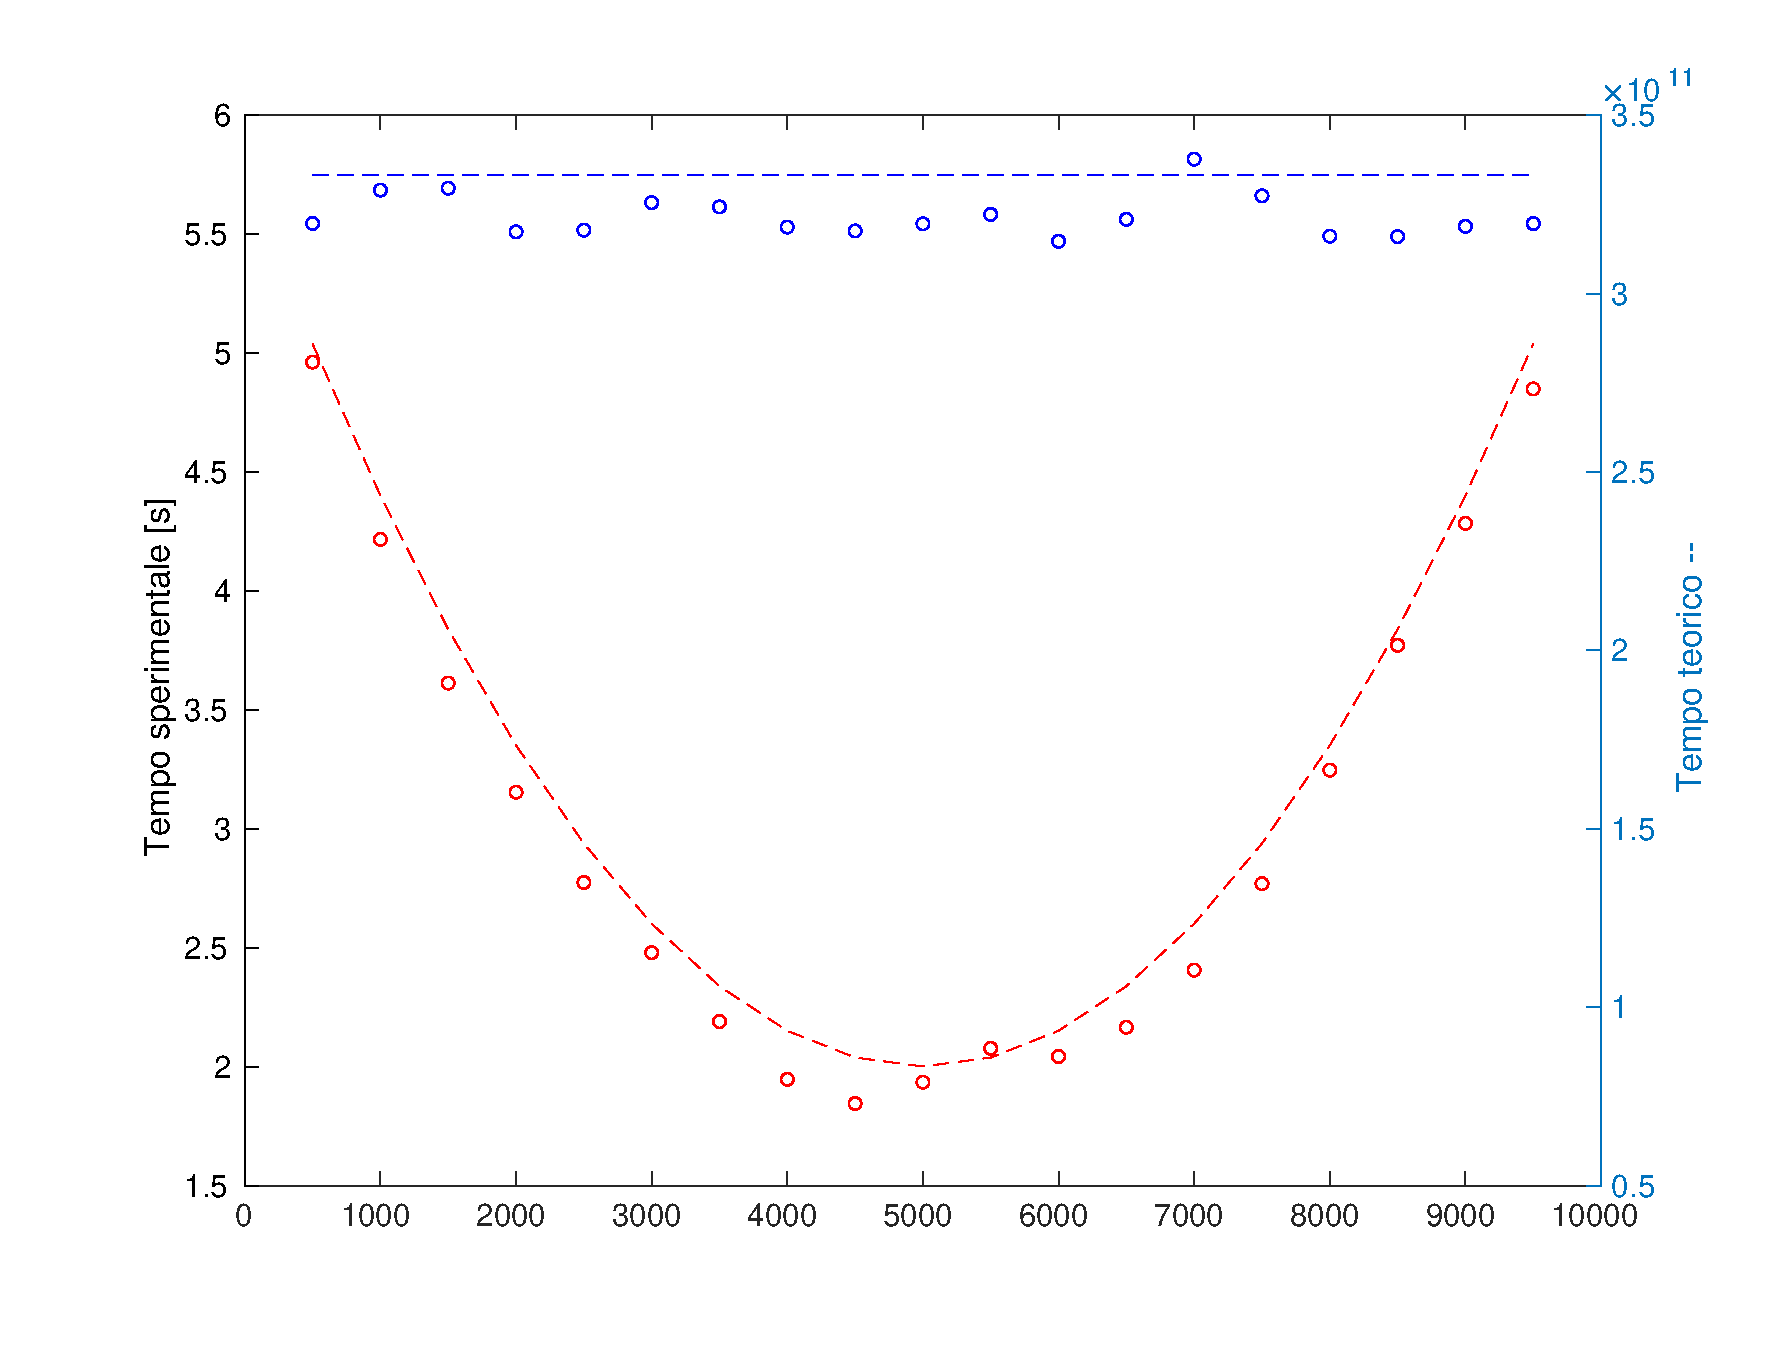
\includegraphics[width=0.71\textwidth]{./Esercizi_images/untitled5.eps}
\end{center}

\clearpage
\subsection*{Vettori, matrici e sistemi lineari - 11}
Come richiesto, vengono generalizzati esercizi 8-10 considerando una matrice triangolare a blocchi $q \times q$ costituita, per semplicità, da blocchi quadrati di dimensione $n/q$.

\begin{lstlisting}
	n = factorial(6);
	asseq = divisors(n);
	res = zeros(n,5); %naif_vero, naif_teo, smart_vero, smart_teo, norma diff
	for q = asseq
		%Definisco dimensione caratteristica
		d = n/q;
		%Genero la matrice A come cell array di matrici quadrate di double
		Acell = repmat({zeros(d)},q,q);
		
		for i=1:q
			for j=i:q
				Acell(i,j) = {rand(d)};
			end
		end
		
		%Per il primo caso ho bisogno di generare tutta la matrice di double
		%Inoltre mi serve anche per definire il vettore dei termini noti
		A = cell2mat(Acell); 
		
		%Calcolo vettore termini noti
		b = A*ones(n,1);
		
		%PRIMO CASO
		tic;
		%x_naif = A\b;
		x_naif = GAUSS_ELIM(A,b);
		res(q,1) = toc;
		res(q,2) = n^3/3+n^2/2;
		clear A;                %Libero memoria
		
		%SECONDO CASO
		x_smart = repmat({zeros(d)},q,1);
		tic;
		for j=q:-1:1
			noto = b((d*(j-1)+1):(d*j));      
				for k=q:-1:(j+1)
					noto = noto - Acell{j,k}*x_smart{k};
				end
			%x_smart{j} = Acell{j,j}\noto;
			x_smart{j} = GAUSS_ELIM(Acell{j,j},noto);
		end
		res(q,3) = toc;
		res(q,4) = n^3/(3*q^2)+n^2/2;
		
		%Controllo risultati
		res(q,5) = norm(x_naif-cell2mat(x_smart),Inf);
	end
	%% PLOTS
	figure();
	yyaxis left
	semilogx(asseq,res(asseq,1),'ob',asseq,res(asseq,3),'or');
	yyaxis right
	semilogx(asseq,res(asseq,2),'--b',asseq,res(asseq,4),'--r');
	legend({'naif','smart'})
	figure();
	loglog(asseq,res(asseq,5),'og');
\end{lstlisting}

\includepdf{./Esercizi_images/untitled6.eps}
\includepdf{./Esercizi_images/untitled7.eps}

\end{document}
